\subsection{Sample design and coverage}\label{app:flow-design}

\Cref{tab:flow-design} lists the strata of the trade sample. The design weight of an event is
its stratum's frame-to-sample event ratio, times $L_e/20$ when the event has $L_e>20$ traded
legs. Sports leagues are identified from the series ticker. ``Other sports'' collects the
remaining leagues, including motor racing, minor soccer and basketball leagues, table tennis
and the Ballon d'Or.

\begin{table}[htbp]
\centering
\begin{threeparttable}
\caption{Sampling frame and stratified sample of the trade-level analysis}\label{tab:flow-design}
\small
\begin{tabular}{lrrrrr}
\toprule
 & \multicolumn{2}{c}{Frame} & \multicolumn{2}{c}{Sample} & \\
\cmidrule(lr){2-3}\cmidrule(lr){4-5}
Stratum & Events & Markets & Events & Markets & Weight per event \\
\midrule
% source: data/research/flb_flow/sample_plan.json
%BEGIN:design
% source: data/research/flb_flow (generated by flb_flow tex)
Combat & 1,295 & 4,688 & 60 & 208 & 21.6 \\
Cricket & 1,154 & 3,463 & 60 & 213 & 19.2 \\
Esports & 32,301 & 67,181 & 150 & 306 & 215.3 \\
Golf & 779 & 12,229 & 40 & 231 & 19.5 \\
MLB & 22,948 & 231,556 & 100 & 624 & 229.5 \\
NBA & 3,935 & 61,082 & 50 & 609 & 78.7 \\
NCAAF & 11,871 & 126,743 & 80 & 891 & 148.4 \\
NFL & 7,995 & 99,542 & 60 & 491 & 133.2 \\
NHL & 4,621 & 44,803 & 60 & 375 & 77.0 \\
Other sports & 43,694 & 147,595 & 150 & 475 & 291.3 \\
Soccer & 32,087 & 134,290 & 120 & 473 & 267.4 \\
Tennis & 30,489 & 65,940 & 150 & 318 & 203.3 \\
WNBA & 2,646 & 19,812 & 60 & 488 & 44.1 \\
Entertainment & 1,160 & 12,095 & 260 & 2,492 & 4.5 \\
Mentions & 349 & 7,230 & 120 & 2,048 & 2.9 \\
Politics & 801 & 4,589 & 260 & 1,515 & 3.1 \\
Science \& Tech & 426 & 3,200 & 220 & 1,615 & 1.9 \\
Weather & 12,303 & 82,218 & 300 & 1,957 & 41.0 \\
%END:design
\bottomrule
\end{tabular}
\begin{tablenotes}\footnotesize
\item Frame: settled, non-financial Kalshi markets that closed 15~August--31~October 2026 and
traded at least once. Events are drawn uniformly at random within each stratum (seed
20261111). Weight per event: frame events divided by sample events.
\end{tablenotes}
\end{threeparttable}
\end{table}

\begin{table}[htbp]
\centering
\begin{threeparttable}
\caption{Coverage of the main trade sample by group}\label{tab:flow-coverage}
\footnotesize
\setlength{\tabcolsep}{4pt}
\begin{tabular}{@{}lrrrrrrrr@{}}
\toprule
 & & & & Taker & Contracts & Taker \$ & Dropped & Complete \\
Group & Markets & Events & Prints & orders & (m) & (m) & (\%) & (\%) \\
\midrule
% source: data/research/flb_flow/summary.json (coverage)
%BEGIN:coverage
% source: data/research/flb_flow (generated by flb_flow tex)
Sports & 5,026 & 1,003 & 1,529,207 & 994,330 & 191.84 & 92.30 & 40.9 & 100 \\
Weather & 1,720 & 297 & 203,699 & 96,491 & 4.03 & 1.79 & 17.7 & 100 \\
Politics & 1,489 & 258 & 339,908 & 213,216 & 37.93 & 17.81 & 10.2 & 100 \\
Entertainment & 2,435 & 258 & 278,713 & 161,512 & 22.48 & 10.10 & 9.4 & 100 \\
Mentions & 1,921 & 119 & 245,400 & 126,128 & 9.21 & 3.07 & 43.5 & 100 \\
Science \& Tech & 1,573 & 216 & 88,190 & 51,857 & 11.19 & 6.59 & 3.3 & 100 \\
%END:coverage
\bottomrule
\end{tabular}
\begin{tablenotes}\footnotesize
\item Counts after the pre-resolution filter. Taker \$ is the taker side's notional,
$\sum n\q$. Dropped: the share of all fetched prints removed by the filter. Complete: the median
across markets of contracts printed over the market's reported volume.
\end{tablenotes}
\end{threeparttable}
\end{table}

\subsection{Choosing the pre-resolution cut}\label{app:flow-preres}

% source: data/research/flb_flow/summary.json (pre_resolution)
\Cref{tab:flow-preres} motivates the cut-offs. In sports the share of contracts traded at
$\le3\cents$ or $\ge97\cents$ is 3--10\% more than half an hour before the close. It then rises
to about 20\% at 10--30 minutes, about 35\% at 5--10 minutes and 65--75\% in the last five
minutes. These are games that are already decided and sweeps after the final whistle. In
non-sports markets that closed early, the share jumps from 22--35\% to 72--89\% in the last hour,
while the event that closed the market unfolds. The four-hour cut is deliberately wider than
that, because the moment the event occurred is not observed. In markets that closed on schedule,
extreme prices are common at every horizon. They come from the far legs of multi-outcome events,
which are genuine longshots, so they are kept.

\begin{table}[htbp]
\centering
\begin{threeparttable}
\caption{Share of contracts traded at extreme prices by minutes before the close (\%)}\label{tab:flow-preres}
\footnotesize
\begin{tabular}{@{}lrrrrr@{}}
\toprule
 & \multicolumn{2}{c}{Sports} & \multicolumn{2}{c}{Non-sports} & Share of \\
\cmidrule(lr){2-3}\cmidrule(lr){4-5}
Minutes before close & On schedule & Early & On schedule & Early & volume \\
\midrule
% source: data/research/flb_flow/summary.json (pre_resolution)
%BEGIN:preres
% source: data/research/flb_flow (generated by flb_flow tex)
0--5 & $75$ & $65$ & $61$ & $89$ & 5.2 \\
5--10 & $35$ & $34$ & $68$ & $86$ & 4.8 \\
10--30 & $22$ & $18$ & $54$ & $80$ & 15.6 \\
30--60 & $9$ & $10$ & $62$ & $72$ & 15.0 \\
60--240 & $4$ & $3$ & $67$ & $22$ & 32.5 \\
$>240$ & $5$ & $8$ & $45$ & $35$ & 26.8 \\
%END:preres
\bottomrule
\end{tabular}
\begin{tablenotes}\footnotesize
\item All fetched prints of the main sample, before any filter. Extreme: YES price $\le3\cents$
or $\ge97\cents$; contract-weighted, unweighted by design. Closed early: closed more than 30
minutes before the scheduled expiration. Share of volume: the window's share of all contracts.
\end{tablenotes}
\end{threeparttable}
\end{table}

\subsection{Returns by price bucket}\label{app:flow-buckets}

\Cref{tab:flow-buckets} and \cref{fig:flow-roles-groups} give pooled, design-weighted returns by
price bucket for both roles, overall and by group. \Cref{tab:flow-yesno} splits takers by the
side they bought. The pooled longshot cells are dominated by a few upsets
(\cref{sec:res-flow-roles}); the per-stratum medians in the main text are the robust summary.

\begin{figure}[htbp]
\centering
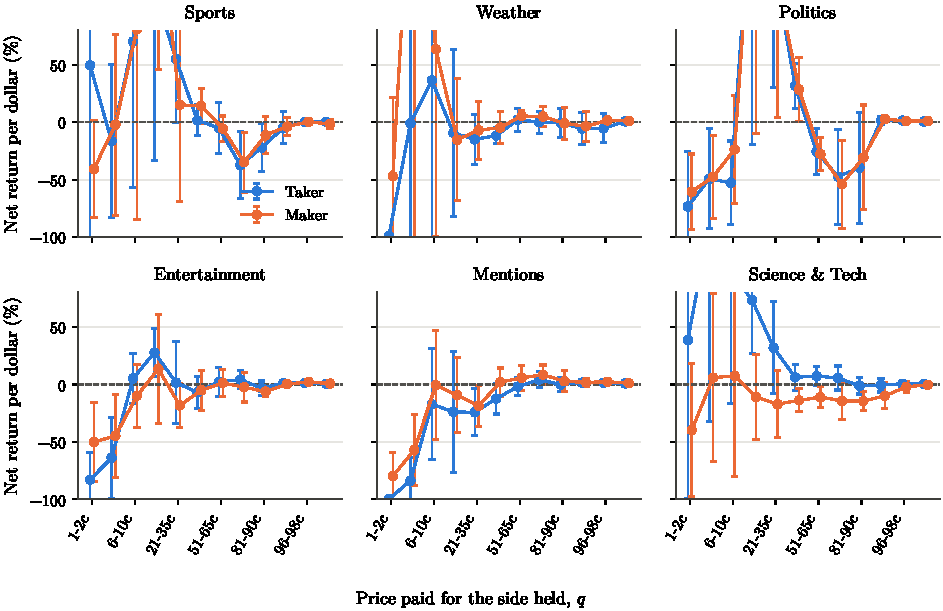
\includegraphics[width=\textwidth]{figures/fig_flow_roles_groups.pdf}
\caption{Takers against makers by price bucket and group. Net return per dollar
(dollar-weighted, after each role's fee) of taker and maker positions, by the price of the side
held, with 95\% confidence intervals clustered by event. Main sample, design-weighted.}\label{fig:flow-roles-groups}
% source: data/research/flb_flow/tables/roles_bucket.csv
\end{figure}

\begin{table}[htbp]
\centering
\begin{threeparttable}
\caption{Taker and maker returns by the price of the side held}\label{tab:flow-buckets}
\footnotesize
\setlength{\tabcolsep}{4pt}
\begin{tabular}{@{}lrrrrr@{}}
\toprule
 & Taker & \multicolumn{2}{c}{Taker} & \multicolumn{2}{c}{Maker} \\
\cmidrule(lr){3-4}\cmidrule(lr){5-6}
Side price $\q$ & share (\%) & Gross (\cents) & Net (\%/\$) & Gross (\cents) & Net (\%/\$) \\
\midrule
% source: data/research/flb_flow/tables/roles_bucket.csv
%BEGIN:roles_bucket
% source: data/research/flb_flow (generated by flb_flow tex)
1--2\cents & $56$ & $+0.48$ $(0.4)$ & $+29.5$ $(0.3)$ & $-0.55$ $(-2.1)$ & $-41.9$ $(-2.2)$ \\
3--5\cents & $56$ & $-0.46$ $(-0.3)$ & $-17.2$ $(-0.5)$ & $+0.06$ $(0.0)$ & $+0.8$ $(0.0)$ \\
6--10\cents & $64$ & $+6.18$ $(1.2)$ & $+68.3$ $(1.1)$ & $+6.40$ $(1.0)$ & $+78.7$ $(1.0)$ \\
11--20\cents & $56$ & $+19.67$ $(1.5)$ & $+113.3$ $(1.5)$ & $+31.02$ $(2.4)$ & $+183.1$ $(2.6)$ \\
21--35\cents & $46$ & $+17.22$ $(2.2)$ & $+54.7$ $(2.0)$ & $+4.77$ $(0.4)$ & $+15.1$ $(0.4)$ \\
36--50\cents & $46$ & $+2.29$ $(0.7)$ & $+1.5$ $(0.2)$ & $+6.54$ $(1.9)$ & $+14.1$ $(1.8)$ \\
51--65\cents & $58$ & $-1.40$ $(-0.2)$ & $-5.0$ $(-0.5)$ & $-2.93$ $(-0.9)$ & $-5.5$ $(-1.0)$ \\
66--80\cents & $49$ & $-26.70$ $(-2.3)$ & $-37.2$ $(-2.5)$ & $-25.62$ $(-2.5)$ & $-34.7$ $(-2.6)$ \\
81--90\cents & $41$ & $-17.95$ $(-2.0)$ & $-21.9$ $(-2.0)$ & $-9.49$ $(-1.4)$ & $-11.2$ $(-1.4)$ \\
91--95\cents & $39$ & $-4.02$ $(-0.6)$ & $-4.8$ $(-0.7)$ & $-3.40$ $(-0.9)$ & $-3.7$ $(-0.9)$ \\
96--98\cents & $44$ & $+0.30$ $(0.3)$ & $+0.1$ $(0.1)$ & $+0.41$ $(0.4)$ & $+0.4$ $(0.3)$ \\
99\cents & $42$ & $+0.47$ $(2.5)$ & $+0.4$ $(2.1)$ & $-1.17$ $(-0.7)$ & $-1.2$ $(-0.7)$ \\
%END:roles_bucket
\bottomrule
\end{tabular}
\begin{tablenotes}\footnotesize
\item Main sample, all groups, design-weighted. Each print contributes a taker position at $\q$
and a maker position at $1-\q$, and both are sorted by the price of the side held. Taker share:
the takers' share of the contracts held at that price. Gross: contract-weighted
\eqref{eq:flow-c} with $\fee=0$, in cents. Net: dollar-weighted \eqref{eq:flow-d} after fees, in
percent. $t$-statistics clustered by event are in parentheses.
\end{tablenotes}
\end{threeparttable}
\end{table}

\begin{table}[htbp]
\centering
\begin{threeparttable}
\caption{YES-takers against NO-takers at equal side price}\label{tab:flow-yesno}
\footnotesize
\begin{tabular}{lrrrr}
\toprule
Taker price $\q$ & YES share (\%) & YES-taker, \%/\$ & NO-taker, \%/\$ & Difference \\
\midrule
% source: data/research/flb_flow/tables/yesno_cells.csv, yesno_diff.csv, yesno_share.csv
%BEGIN:yesno
% source: data/research/flb_flow (generated by flb_flow tex)
1--2\cents & $79$ & $+57.3$ $(0.5)$ & $-90.8$ $(-21.0)$ & $+148.1$ $(1.2)$ \\
3--5\cents & $85$ & $-14.2$ $(-0.4)$ & $-33.3$ $(-0.9)$ & $+19.0$ $(0.4)$ \\
6--10\cents & $85$ & $+67.0$ $(1.0)$ & $+75.3$ $(0.9)$ & $-8.3$ $(-0.1)$ \\
11--20\cents & $85$ & $+124.8$ $(1.5)$ & $+48.4$ $(1.0)$ & $+76.4$ $(0.8)$ \\
21--35\cents & $78$ & $+57.1$ $(1.8)$ & $+46.5$ $(2.5)$ & $+10.6$ $(0.4)$ \\
36--50\cents & $73$ & $-6.3$ $(-0.6)$ & $+23.2$ $(1.4)$ & $-29.5$ $(-1.3)$ \\
51--65\cents & $74$ & $-10.4$ $(-0.6)$ & $+11.2$ $(1.2)$ & $-21.6$ $(-1.0)$ \\
66--80\cents & $71$ & $-42.9$ $(-2.7)$ & $-22.9$ $(-1.8)$ & $-20.1$ $(-2.3)$ \\
81--90\cents & $62$ & $-31.7$ $(-2.5)$ & $-5.9$ $(-1.1)$ & $-25.8$ $(-3.2)$ \\
91--95\cents & $48$ & $-9.1$ $(-0.9)$ & $-0.7$ $(-0.2)$ & $-8.4$ $(-1.4)$ \\
96--98\cents & $45$ & $+0.1$ $(0.1)$ & $+0.1$ $(0.1)$ & $-0.0$ $(-0.0)$ \\
99\cents & $53$ & $+0.4$ $(1.7)$ & $+0.4$ $(1.3)$ & $+0.0$ $(0.1)$ \\
%END:yesno
\bottomrule
\end{tabular}
\begin{tablenotes}\footnotesize
\item Main sample, all groups, taker positions only, design-weighted. Net return per dollar is
dollar-weighted \eqref{eq:flow-d}, in percent. YES share: the share of taker contracts at that
price bought as YES. Difference: YES minus NO, in percentage points, with an event-clustered $t$
that accounts for shared events.
\end{tablenotes}
\end{threeparttable}
\end{table}

\subsection{Trade size by sector}\label{app:flow-size}

\Cref{tab:flow-size-sector} repeats \cref{tab:flow-size} separately for sports and non-sports
markets. The longshot share of small orders is twice as high outside sports.

\begin{table}[htbp]
\centering
\begin{threeparttable}
\caption{Taker flow and returns by order size, sports and non-sports}\label{tab:flow-size-sector}
\footnotesize
\setlength{\tabcolsep}{4pt}
\begin{tabular}{@{}llrrrrrr@{}}
\toprule
 & & \multicolumn{2}{c}{Share of taker} & Share at & Mean & \multicolumn{2}{c}{Taker net return per dollar} \\
\cmidrule(lr){3-4}\cmidrule(lr){7-8}
Sector & Order size & orders & contracts & $\q\le10\cents$ & $\q$ (\cents) & Longshots & Favourites \\
\midrule
% source: data/research/flb_flow/tables/size_shares_sector.csv, size_side_sector.csv
%BEGIN:size_sector
% source: data/research/flb_flow (generated by flb_flow tex)
Sports & $\le$\$10 & $51.7$ & $4.7$ & $36.3$ & $23$ & $+36.1$ $(0.8)$ & $-2.7$ $(-1.2)$ \\
 & \$10--100 & $37.7$ & $20.9$ & $17.0$ & $35$ & $+55.3$ $(1.1)$ & $-1.0$ $(-0.4)$ \\
 & \$100--1k & $9.5$ & $31.8$ & $8.3$ & $47$ & $+27.3$ $(0.6)$ & $-1.4$ $(-0.5)$ \\
 & $>$\$1k & $1.2$ & $42.7$ & $1.2$ & $58$ & $+169.0$ $(1.2)$ & $-3.8$ $(-1.0)$ \\
Non-sports & $\le$\$10 & $67.1$ & $20.7$ & $74.0$ & $13$ & $-35.2$ $(-1.3)$ & $-2.4$ $(-1.1)$ \\
 & \$10--100 & $24.8$ & $32.3$ & $46.4$ & $30$ & $-23.1$ $(-1.0)$ & $-3.4$ $(-1.1)$ \\
 & \$100--1k & $7.0$ & $27.7$ & $21.6$ & $56$ & $-29.7$ $(-1.3)$ & $-0.9$ $(-0.6)$ \\
 & $>$\$1k & $1.1$ & $19.4$ & $2.6$ & $81$ & $-85.1$ $(-4.6)$ & $+0.5$ $(0.6)$ \\
%END:size_sector
\bottomrule
\end{tabular}
\begin{tablenotes}\footnotesize
\item As \cref{tab:flow-size}, separately for sports and non-sports markets. Shares are in
percent within the sector. Returns are dollar-weighted \eqref{eq:flow-d} after the taker fee,
with event-clustered $t$-statistics in parentheses.
\end{tablenotes}
\end{threeparttable}
\end{table}

\subsection{Timing cells}\label{app:flow-timing}

\Cref{tab:flow-timing-cells} lists taker flow and returns in every timing and attention cell
used in \cref{sec:res-flow-timing}.

\begin{table}[htbp]
\centering
\begin{threeparttable}
\caption{Taker flow and returns by timing and attention cell}\label{tab:flow-timing-cells}
\footnotesize
\begin{tabular}{@{}lrrrrr@{}}
\toprule
 & Volume & \multicolumn{2}{c}{Taker return per dollar (\%)} & Share at & Orders \\
\cmidrule(lr){3-4}
Cell & share (\%) & Net & Gross & $\q\le10\cents$ (\%) & $\le\$100$ (\%) \\
\midrule
% source: data/research/flb_flow/tables/timing.csv
%BEGIN:timing_cells
% source: data/research/flb_flow (generated by flb_flow tex)
\multicolumn{6}{@{}l}{\emph{Hour of day (ET)}} \\
\quad 00--06 & $8.1$ & $-10.3$ $(-1.7)$ & $-8.2$ $(-1.4)$ & $11.2$ & $89.5$ \\
\quad 06--12 & $11.8$ & $-11.0$ $(-2.3)$ & $-8.9$ $(-1.8)$ & $9.5$ & $89.5$ \\
\quad 12--18 & $41.2$ & $-1.2$ $(-0.2)$ & $+1.3$ $(0.2)$ & $8.8$ & $88.8$ \\
\quad 18--24 & $38.8$ & $+0.9$ $(0.3)$ & $+3.4$ $(1.1)$ & $8.2$ & $89.9$ \\
\multicolumn{6}{@{}l}{\emph{Day}} \\
\quad Weekday & $72.6$ & $+0.7$ $(0.2)$ & $+3.2$ $(0.9)$ & $8.4$ & $89.5$ \\
\quad Weekend & $27.4$ & $-10.2$ $(-2.3)$ & $-8.1$ $(-1.8)$ & $10.0$ & $89.2$ \\
\multicolumn{6}{@{}l}{\emph{Sports game phase}} \\
\quad Pre-game & $33.4$ & $-3.4$ $(-0.4)$ & $-0.9$ $(-0.1)$ & $5.3$ & $91.6$ \\
\quad In play & $66.6$ & $-2.6$ $(-1.1)$ & $-0.3$ $(-0.1)$ & $8.5$ & $88.1$ \\
\multicolumn{6}{@{}l}{\emph{Sports game start}} \\
\quad Before 19:00 ET & $55.0$ & $-2.7$ $(-0.4)$ & $-0.4$ $(-0.1)$ & $8.7$ & $88.3$ \\
\quad 19:00--23:59 ET & $45.0$ & $-3.1$ $(-1.2)$ & $-0.7$ $(-0.3)$ & $6.0$ & $90.6$ \\
\multicolumn{6}{@{}l}{\emph{Time to scheduled expiry}} \\
\quad $<1$ h & $13.4$ & $-5.2$ $(-2.4)$ & $-3.2$ $(-1.4)$ & $9.7$ & $87.4$ \\
\quad 1--6 h & $70.2$ & $-0.4$ $(-0.1)$ & $+2.1$ $(0.6)$ & $7.5$ & $88.1$ \\
\quad 6--24 h & $10.7$ & $-1.5$ $(-0.1)$ & $+1.1$ $(0.1)$ & $9.2$ & $92.8$ \\
\quad 1--7 days & $4.5$ & $-26.8$ $(-2.2)$ & $-25.2$ $(-2.0)$ & $17.3$ & $96.1$ \\
\quad $>7$ days & $1.3$ & $-1.1$ $(-0.4)$ & $+0.9$ $(0.3)$ & $43.9$ & $90.1$ \\
\multicolumn{6}{@{}l}{\emph{Market age}} \\
\quad First 24 h & $23.0$ & $-5.8$ $(-1.6)$ & $-3.7$ $(-1.0)$ & $10.7$ & $86.3$ \\
\quad Later & $77.0$ & $-1.4$ $(-0.3)$ & $+1.1$ $(0.3)$ & $8.3$ & $90.2$ \\
\multicolumn{6}{@{}l}{\emph{Past-hour volume vs own average}} \\
\quad $<0.5\times$ & $2.7$ & $-13.8$ $(-2.0)$ & $-11.7$ $(-1.7)$ & $27.2$ & $92.0$ \\
\quad $0.5$--$3\times$ & $4.1$ & $-12.4$ $(-1.1)$ & $-10.5$ $(-0.9)$ & $16.0$ & $93.9$ \\
\quad $3$--$10\times$ & $7.2$ & $-12.2$ $(-1.4)$ & $-10.2$ $(-1.1)$ & $11.5$ & $93.3$ \\
\quad $\ge10\times$ & $86.0$ & $-0.7$ $(-0.2)$ & $+1.8$ $(0.5)$ & $6.9$ & $88.4$ \\
\multicolumn{6}{@{}l}{\emph{Event volume}} \\
\quad Below top decile & $14.1$ & $-3.3$ $(-1.2)$ & $-1.1$ $(-0.4)$ & $12.4$ & $89.3$ \\
\quad Top decile (marquee) & $85.9$ & $-2.3$ $(-0.6)$ & $+0.2$ $(0.0)$ & $8.3$ & $89.4$ \\
%END:timing_cells
\bottomrule
\end{tabular}
\begin{tablenotes}\footnotesize
\item Main sample, all groups, taker positions, design-weighted. Volume share: the cell's share
of taker contracts within the panel. Returns are dollar-weighted \eqref{eq:flow-d}, with
event-clustered $t$-statistics in parentheses. Share at $\q\le10\cents$: the share of taker
contracts bought at a longshot price. Orders $\le\$100$: the share of taker orders with a
notional of at most \$100. Game phase and start time cover sports games with a known scheduled
start. The past-hour volume ratio needs six hours of trading history.
\end{tablenotes}
\end{threeparttable}
\end{table}
